\chapter{Senzory}
\label{sec:Sensors}
\

Platforma FRDM-K66F obsahuje tři senzory, které tvoří 9osou IMU jednotku.
NXP FXOS8700CQ slouží jako akcelerometr i magnetometr a NXP FXAS21002 jako gyroskop.
Tyto~senzory komunikují s platformou pomocí $I^2C$ \cite{frdmk66UserGuide}.

\section{NXP FXOS8700CQ}\

\textbf{NXP FXOS8700CQ} je pokročilý 6osý senzor, který kombinuje funkce 3osého
akcelerometru a 3osého magnetometru v jednom čipu. Akcelerometr v senzoru
FXOS8700CQ má nastavitelné rozsahy ±2 g, ±4 g, ±8 g s 14bitovým rozlišením, zatímco
magnetometr poskytuje 16bitové rozlišení s~rozsahem ±1200 µT na osu. Pro komunikaci
podporuje $I^2C$ a $SPI$ rozhraní. Má dva piny pro~přerušení a podporuje odesílat data
rychlosti až 800 Hz pro každý senzor případně 400 Hz v~hybridním režimu.
Tato~integrace umožňuje zařízení zachytit komplexní data o svém pohybu a orientaci
vůči zemskému gravitačnímu a magnetickému poli. Orientace akcelerometru a
magnetometru je na~obrázku \ref{fig:FXOS_Orientation} \cite{FXOS8700CQ}.

\section{NXP FXAS21002}\

\textbf{NXP FXAS21002} je vysoce výkonný 3osý senzor, který poskytuje data o úhlové
rychlosti zrychlení. Tento senzor má nastavitelné rozsahy ±250, ±500, ±1000, a
±2000 stupňů za sekundu s~16bitovým rozlišením. Pro komunikaci podporuje $I^2C$ a
SPI rozhraní. Obsahuje dva piny pro~přerušení a podporuje odesílat data rychlosti až
800 Hz, což umožňuje zařízení detekovat rotace kolem svých os. Orientace gyroskopu
je zobrazena na obrázku \ref{fig:FXAS_Orientation} \cite{FXAS21002}.

\begin{figure}[ht]
    \centering
	\begin{subfigure}{0.35\textwidth}
	    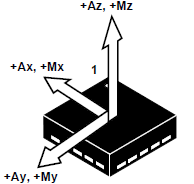
\includegraphics[width = \textwidth]{Figures/FXOS_Orientation.png}
        \label{fig:FXOS_Orientation}
        \caption{NXP FXOS8700CQ orientace \cite{FXOS8700CQ}.}
	\end{subfigure}
    \begin{subfigure}{0.35\textwidth}
        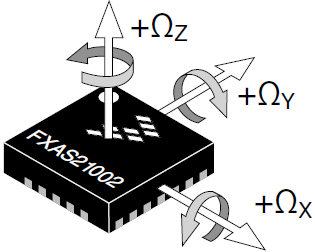
\includegraphics[width = \textwidth]{Figures/FXAS_Orientation.png}
        \label{fig:FXAS_Orientation}
         \caption{NXP FXAS21002 orientace \cite{FXAS21002}.}
    \end{subfigure}
	\caption{Orientace senzorů.}
\end{figure}

\section{Komunikace se senzory}\

Pro komunikaci se senzory je použita \textbf{$I^2C$ sběrnice}. $I^2C$ sběrnice má 2
vodiče pro všechny zařízení, SDA a SCL. \textbf{SDA} je datová linka, která
přenáší data mezi zařízeními, zatímco \textbf{SCL} je hodinová linka, která
synchronizuje přenos dat. Na sběrnici existuje jedno zařízení, které je
\textbf{master}, a může komunikovat s zařízeními, které jsou \textbf{slave}. Master
zařízení generuje hodinový signál a určuje, kdy se data posílají a přijímají. Každé
zařízení na~sběrnici má svou vlastní adresu, která je 7 bitů dlouhá. Oba vodiče jsou
aktivní v logické 0, což znamená, že v klidovém stavu jsou oba vodiče v logické 1.
Když je zařízení připojeno k systému, musí být připojeno na zemi, aby mohlo
komunikovat.

Přenos na sběrnice vždy začíná START sekvencí a končí STOP sekvencí, viz. obrázek
\ref{fig:I2C_FRAME}. Ty~jsou generovány master zařízením. \textbf{START} sekvence je
definovaná jako přechod z logické 1 na~logickou 0 na SDA, zatímco na SCL je v
logické 1. \textbf{STOP} sekvence oproti tomu má jako přechod z logické~0
na~logickou 1 na SDA, zatímco na SCL je v logické 1. Sběrnice je obsazena od začátku
START~sekvence až do konce STOP sekvence.

Pro zápis dat na sběrnici je nejprve nutné poslat adresu zařízení, které přijímá
data. Adresa má 7 bitů a poslední bit je R/W, který určuje, zda se jedná o zápis
nebo čtení. Poté jak slave pošle ACK bit (znamení, že je připraven přijmout data),
master posílá data a slave potvrzuje přijetí ACK~bitem.

Čtení dat se podobá zápisu, po odeslání adresy zařízení, které posílá data, se
master přepne do~režimu čtení a slave pošle data, která master potvrdí ACK
bitem \cite{I2C}.

\begin{figure}[!h]
    \centering
    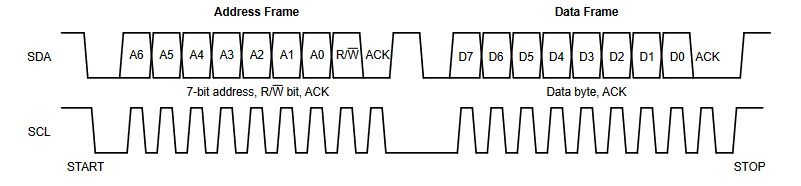
\includegraphics[width = .9\linewidth]{Figures/I2C_FRAME.png}
    \caption{I2C frame\cite{I2C}.}
    \label{fig:I2C_FRAME}
\end{figure}

\section{Konfigurace senzorů}\

Konfiguraci senzorů je probíhá posláním dat na jejich adresy. Adresy
jsou:
\begin{itemize}
    \item NXP FXOS8700CQ - 0x1D;
    \item NXP FXAS21002 - 0x21.
\end{itemize}

\subsection{Konfigurace NXP FXOS8700CQ}\

Pro nastavení NXP FXOS8700CQ bylo nastaveny nasledující registry: CTRL\_REG\_1,
CTRL\_REG\_2, CTRL\_REG\_4, CTRL\_REG\_5, M\_CTRL\_REG\_1, M\_CTRL\_REG\_2,
XYZ\_DATA\_CFG. Adresa registru a hodnoty jsou v tabulce \ref{tab:FXOS8700CQ}.

\begin{table}[!h]
    \centering
	\begin{tabular}{ccc}
        \hline
        \textbf{Adresa} & \textbf{Registr} & \textbf{Hodnota} \\
        \hline
        0x2A            & CTRL\_REG1       & 0x1D             \\
        0x2B            & CTRL\_REG2       & 0x1E             \\
        0x2D            & CTRL\_REG4       & 0x01             \\
        0x2E            & CTRL\_REG5       & 0x00             \\
        0x5B            & M\_CTRL\_REG1    & 0x5F             \\
        0x5C            & M\_CTRL\_REG2    & 0x20             \\
        0x0E            & XYZ\_DATA\_CFG   & 0x01             \\
        \hline
    \end{tabular}
    \caption{Konfigurace NXP FXOS8700CQ\cite{FXOS8700CQ}.}
    \label{tab:FXOS8700CQ}
\end{table}

\begin{itemize}
    \item CTRL\_REG1 je použit pro přepnutí režimu senzoru mezi standby a active.
    Pro jakékoliv změny v registrech je nutné přepnout senzor do standby režimu.
    Pokud všechny registry byly nastaveny, je možné přepnout senzor do active
    režimu, a dále tento registr použit pro nastavení frekvence vzorkování na 50 Hz
    a zapnutí malého šumu.

    \item CTRL\_REG2 je použit pro zapnutí automatického režimu spanku, nízkého
    výkonu ve~spánku a vysokého výkonu v probuzení.

    \item CTRL\_REG4 je použit pro zapnutí data-ready přerušení.

    \item CTRL\_REG5 je použit pro nastavení pinu přerušení na INT2.

    \item M\_CTRL\_REG1 je použit pro zapnutí hybridního režimu,jednorázového
    magnetického resetu a nastavení oversample ratio na 7. V hybridním režimu je
    možné získat data z akcelerometru a magnetometru současně.

    \item M\_CTRL\_REG2 je použit pro zapnutí automatického hybridního režimu
    inkrementu adresy. Co znamená, že po přečtení dat z akcelerometru se začíná čist
    data z magnetometru.

    \item Registr XYZ\_DATA\_CFG je použit pro nastavení rozsahu akcelerometru na ±4
    g \cite{FXOS8700CQ}.
\end{itemize}

\subsection{Konfigurace NXP FXAS21002}\

Pro nastavení NXP FXAS21002 bylo nastaveny nasledující registry: CTRL\_REG0,
CTRL\_REG1, CTRL\_REG2. Adresa registru a hodnoty jsou v tabulce
\ref{tab:FXAS21002}.

\begin{table}[!h]
    \centering
    \begin{tabular}{ccc}
        \hline
        \textbf{Adresa} & \textbf{Registr} & \textbf{Hodnota} \\
        \hline
        0x0D            & CTRL\_REG0       & 0x01             \\
        0x13            & CTRL\_REG1       & 0x13             \\
        0x14            & CTRL\_REG2       & 0x0C             \\
        \hline
    \end{tabular}
    \caption{Konfigurace NXP FXAS21002 \cite{FXAS21002}.}
    \label{tab:FXAS21002}
\end{table}

\begin{itemize}
    \item CTRL\_REG0 je použit pro nastavení rozsahu gyroskopu na ±1000 stupňů za
    sekundu \cite{FXAS21002}.

    \item CTRL\_REG1 je použit pro přepnutí režimu senzoru mezi standby a active.
    Pro jakékoliv změny v registrech je nutné přepnout senzor do standby režimu.
    Pokud všechny registry byly nastaveny, je možné přepnout senzor do active
    režimu, a dále tento registr použit pro nastavení frekvence vzorkování na 50
    Hz \cite{FXAS21002}.

    \item CTRL\_REG2 je použit pro zapnutí data-ready přerušení a nastavení pinu
    přerušení na~INT1 \cite{FXAS21002}.
\end{itemize}

\section{Čtení dat ze senzorů}\

Všechny senzory ukládají hodnoty do 6 registrů. Akcelerometr ukládá informace o
naměřeném zrychlení do registrů 0x01 až 0x06. Gyroskop ukládá informace o naměřeném
úhlovém zrychlení do~registrů 0x01 až 0x06. Magnetometr ukládá informace o naměřeném
magnetickém poli do registrů 0x33 až 0x38. Zde jsou uložené data pro osy X, Y a Z.

Obě zařízení umožňují čist data z více registrů najednou. Pro získání dat stačí jen
začít čtení na první adrese datového registru 0x01. Data se posílají ve formátu big
endian, což znamená, že nejprve je poslán nejvyšší bajt a poté nejnižší bajt.

\section{Výběr senzoru}\

Pro výběr vhodného senzoru byla analyzována data získaná po jízdě vozidla po dráze,
viz. v~kapitole \ref{sec:PlatformControl}. Tato data jsou vizualizována na obrázku
\ref{fig:Sensors}.
\begin{figure}[!h]
    \centering
    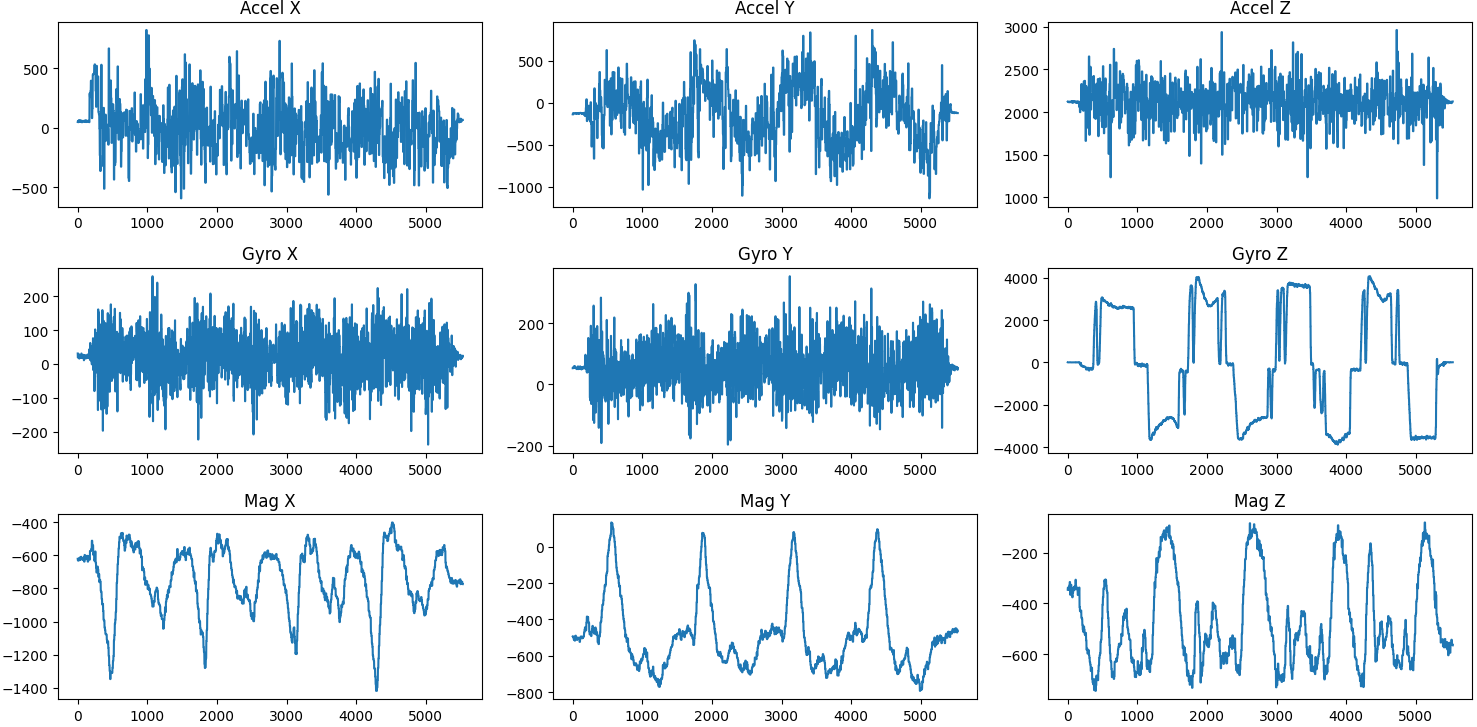
\includegraphics[width = 1\linewidth]{Figures/Sensors.png}
    \caption{Data ze senzorů.}
    \label{fig:Sensors}
\end{figure}

Z obrázku je zřejmé, že otáčení vozidla koresponduje s daty získanými
z akcelerometru na ose $y$ a gyroskopu na ose $z$. Nicméně je třeba poznamenat, že
data z akcelerometru obsahují významný šum, což vyžaduje implementaci vhodného
filtračního algoritmu před dalším zpracováním těchto dat. Dále je třeba zmínit, že
data z magnetometru nelze v tomto případě využít, jelikož jsou negativně ovlivněna
působením motorů vozidla. Možnost přesunutí senzoru magnetometru na méně náchylné
místo myšleno například blíže ke kameře by bylo ideální, avšak v dané konfiguraci
vozidla není proveditelné. Vzhledem k těmto omezením a za účelem optimalizace
rychlosti zpracování bude v~práci použita kombinace dat pouze z akcelerometru a
gyroskopu.

\endinput
